\section{Where does the time go?}\label{sec:exp}
\paragraph{Evaluation design.}
We fixed \(N=16,P=4,Q=14,B=1\) for the primary comparison. In fixed-trace replay, a path returns its archived vote at its recorded output length. A decision is certified when the observed margin beats every assignment of the remaining votes, including unlaunched paths beyond the absolute cap. Both admission gates thus agree on certification and output for fixed votes. A change in the set of co-runners can alter sampled tokens on a real engine. We consider controlled generation and natural generation separately.

We used three previously studied cohorts to audit the bound. AIME 2025 contains 30 problems, each with two disjoint panels, and AMC 2023 supplies 40 second-draw panels. Their unsteered paths come from Qwen3-4B-Base and the same public trajectory publisher. The OlympiadBench cohort \citep{he2024olympiadbench} contains 24 independently selected English integer-answer questions generated with DeepSeek-R1-Distill-Qwen-1.5B. We archived one full reference panel per question. The matched AIME comparison was retrospective. We also evaluated a new GSM8K split \citep{gsm8k}, freezing the comparison, question selection and primary clock before retrieving its trajectories.

For each question, we sum its policy times across its panels and compute \(1-T_{\rm candidate}/T_{\rm reference}\). We average these ratios across questions. A positive percentage favors the candidate. We report the median, the ratio of pooled times, and question-level uncertainty where available. A ratio of pooled times weights long questions more heavily. Requests belonging to one question share input and decision conditions.

\subsection{Calibrating the width clock}
One A800-SXM4-80GB ran DeepSeek-R1-Distill-Qwen-1.5B in BF16 using vLLM 0.8.5. Each of eight randomized blocks included widths 1 through 4 and all three initial contexts. After prefill and an eight-step decode prelude we timed 96 steps between device synchronizations, verifying one new token per active path on every step. We paired first-request seeds across widths, disabled prefix caching and kept all synthetic prompts at the indicated length. A separate full block warmed up the engine.

\begin{table}[tb]\centering
\caption{Measured milliseconds per decode step. Each cell is the median of eight timed windows. The replay uses one row throughout each panel.}\label{tab:cost}
\begin{tabular}{lrrrr}\toprule
Initial context & \(c_1\) & \(c_2\) & \(c_3\) & \(c_4\)\\\midrule
512 & 5.283 & 5.286 & 5.479 & 5.585\\
2,048 & 5.297 & 5.399 & 5.545 & 5.676\\
3,968 & 5.321 & 5.463 & 5.717 & 5.862\\\bottomrule
\end{tabular}
\end{table}
All three median curves violate discrete concavity at $j=2$, as do the individual block estimates at that index in all three contexts. Applying the concave majorant to each median clock bounds the saving over greedy on \emph{every} zero-overrun panel by 1.823\%, 0.452\% and 1.015\% at 512, 2,048 and 3,968 tokens, respectively. The explicit $j=2$ witness in the proof yields modeled savings of 1.776\%, 0.408\% and 1.015\%. These are worst-case results for each specified clock. The clock omits prefill and queueing and extrapolates a cached-decode price across every step of a panel.

\subsection{Headroom after indexed admission}
Table~\ref{tab:floor} gives the ceiling on what \emph{any} compliant timing policy could save relative to indexed greedy in the specified clock. Merely charging the minimum step price for \(V_G\) suggests room for five to eight percent at the longest calibration length. Requiring the aggregate work of each potentially decisive subset accounts for most of the difference. The ordered-work and optimistic completion constraints tighten the result further, particularly on AMC.

\begin{table}[tb]\centering
\caption{Question-mean ceiling on decision time saved over indexed greedy (\%). Fixed 3,968-token clock. Work uses the total length of each candidate's completed paths. Full uses Theorem~\ref{th:floor}.}\label{tab:floor}
\small\setlength{\tabcolsep}{4pt}
\begin{tabular}{lrrrr}\toprule
Cohort & Panels & \(V_G\min c_k\) & Work & Full\\\midrule
AIME25 & 60 & 5.571 & 0.287 & 0.216\\
AMC23 & 40 & 5.578 & 0.910 & 0.424\\
OlympiadBench & 24 & 7.903 & 0.549 & 0.215\\\bottomrule
\end{tabular}
\end{table}
The full ceilings at 512 prompt tokens were 0.413\%, 0.528\% and 0.181\% in the same cohort order. At 2,048 they were 0.117\%, 0.268\% and 0.139\%. These upper bounds describe entire questions under each fixed clock. A scheduler cannot realize the LP's choices merely by solving it after some votes arrive. Its construction uses the final works and votes of the panel and may combine occupancies that no schedule can attain.

We also let each width price independently vary between its smallest and largest 96-step block average at 3,968 tokens. For any fixed clock in this box the four cohort ceilings are 0.296\%, 0.500\%, 0.235\% and 0.845\% (GSM8K last). Even allowing time-varying prices inside the box gives 0.509\%, 0.713\%, 0.482\% and 1.034\%. These bounds assume per-step prices stay inside the observed range of block averages. Appendix~\ref{app:box} describes the calculation.

\subsection{A new archive split tests both comparisons}
Before reading any GSM8K rollout payload, we hash-ranked all 53 eligible first-draw unsteered shards in the pinned Reasoning Cues release and froze the eight selected shards, parser and policy code. They yielded 200 complete questions, each with sixteen distinct indexed paths in source order, with no incomplete selected group. A truncated response or missing final boxed answer abstained. This split changes the problem family while retaining the AIME and AMC rollout publisher and model.

Indexed admission changed the vector of launch times on 138 questions. At the prespecified longest-context clock, it shortened 109 questions and slowed 28. Its average time saving against buffered admission was 8.71\% (95\% question-bootstrap interval 6.61--11.02\%). The median was 0.14\% and pooling elapsed times gave 18.72\%. Mean generated work fell by 1.58\%. Under equal virtual rates \(G\) dominates the comparator's decision time. Its occasional slower physical time follows from the measured cost of wider concurrency. Under the shorter-context clocks the mean saving remained positive (Appendix~\ref{app:data}).

\paragraph{Which information accounts for the gain?} The buffered gate uses only contiguous-prefix votes for admission. Against a gate using the completed-index mask and all returned vote counts, indexed admission saved 0.67\% (95\% interval 0.25--1.22\%). Also retaining the prefix's vote-to-index pairs reduced it to 0.30\% (0.07--0.61\%). Both controls were retrospective. With each question's buffered time as a common denominator, incorporating the out-of-prefix votes without assigning them to individual indices saved 8.41 percentage points on average. Resolving their indices added 0.30 points, together accounting for the 8.71\% saving. The prefix-plus-multiset and indexed gates differed in dispatch on 22 of 200 archive questions and agreed on all 64 question--limit device replays. The live comparisons below timed buffered and indexed admission. Appendix~\ref{app:bag} defines the stronger gate.

We compared three executable withholding policies with indexed greedy. Let \(g\) be the current margin, \(R\) the remaining votes, and \(a\) the requests already running before refill. If \(a>0\) and \(g+2a>R\), those active requests could lock the vote by all favoring a current leader. The repeated-wait rule then withholds the last newly admissible path until the next completion. It reevaluates this test at each opportunity. A timed version postpones only at the first such event, for at most eight virtual steps or until the next completion. An unconditional control applies the same timer at the first eligible event. All methods start with the usual full admissible width and keep at least one request running.

\begin{table}[tb]\centering
\caption{GSM8K question-mean time savings, in percent. Positive favors the candidate. Bootstrap intervals resample 200 questions. The last row uses future information to select one postponement or leave the panel alone.}\label{tab:gsm}
\small\setlength{\tabcolsep}{3pt}
\begin{tabular}{lrr}\toprule
Candidate vs.\ reference & Mean & 95\% interval\\\midrule
Indexed vs.\ buffered & 8.71 & [6.61, 11.02]\\
Indexed vs.\ unordered & 0.67 & [0.25, 1.22]\\
Indexed vs.\ prefix + unordered & 0.30 & [0.07, 0.61]\\
Repeat wait vs.\ indexed & $-73.24$ & [$-143.45$, $-20.24$]\\
One timed wait vs.\ indexed & $-0.30$ & [$-0.39$, $-0.22$]\\
Timed control vs.\ indexed & $-0.22$ & [$-0.30$, $-0.15$]\\
Best single wait vs.\ indexed & 0.115 & [0.089, 0.142]\\\bottomrule
\end{tabular}
\end{table}
The eligibility test identifies when a lock \emph{could} occur. It does not imply that the active path will return soon or provide the decisive vote. Repeated waiting slowed 126 questions, improved 39 and tied on the rest. Pooling time gave a 47.00\% increase, compared with the 73.24\% question-mean increase. A single bounded wait contained that loss. Neither executable timed policy reached the prespecified 1\% mean saving with a positive bootstrap lower limit.

To isolate the value of predicting the correct instant, we enumerated every eligible noninitial refill on each greedy run. On one such event we withheld the last admissible launch until the next completion, then resumed greedy admission. Every policy performing at most one such intervention shares all earlier events with the corresponding greedy run. Thus choosing the fastest alternative in hindsight, including the unaltered schedule, gives the exact optimum within this restricted family. This comparison saved time on 168 of the 200 questions yet contributed only 0.115\% on average. A subsequent application of the certificate-work relaxation bounded the improvement of \emph{all} safe timing strategies by 0.738\% at the same clock. This all-strategies GSM8K analysis was added after the frozen comparison. At 512 and 2,048 tokens the corresponding ceilings were 0.760\% and 0.457\%. The two estimates bracket the foresighted optimizer's attainable savings, with the lower endpoint witnessed by a schedule and the upper endpoint supplied by a relaxation.

\begin{figure*}[t]
\centering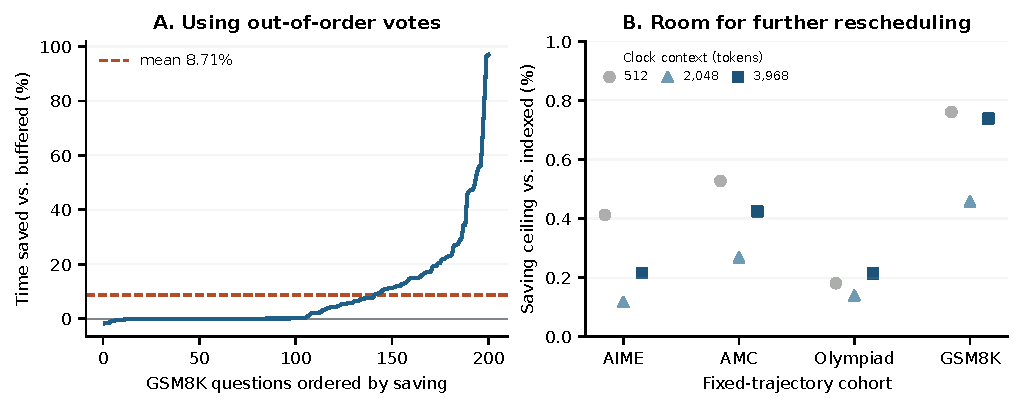
\includegraphics[width=.96\textwidth]{evidence.pdf}
\caption{Two comparisons under fixed service clocks. Left, per-question change in modeled time from using all indexed votes for admission instead of only the contiguous prefix, at the 3,968-token clock. The dashed line is the question mean. Right, the ceiling on mean time savings of any legal scheduler over indexed greedy in each cohort, computed separately with each A800 width-price curve. The two vertical axes have different references and scales.}\label{fig:evidence}
\end{figure*}
Figure~\ref{fig:evidence} shows the heterogeneity in the admission comparison. The typical question changed little, while a subset benefited enough to lift the mean. Across all four cohorts every fixed clock left less than one percent average headroom after indexed admission.

\subsection{Controlled measurements in a decoding engine}
On the 24 OlympiadBench questions we paired the indexed and buffered policies on an A800 by holding the per-path generation lengths and released votes fixed. Each policy issued real vLLM requests and returned on certification or quota exhaustion. We separately sampled natural answers with matched path seeds. In the fixed-work runs the two policies performed every reservation, launch, completion and cancellation at the same engine step on all 24 pairs. Each generated 1,114,134 tokens in total. Their average wall times differed by 0.14\% despite identical dispatches. The natural comparison gave 0.12\% savings (95\% question interval $-0.06$ to 0.32\%). Each condition was timed once per question, so this analysis cannot isolate cross-session timing variance. On fixed votes nine decisions were certified at or before fourteen launches. All 24 capped answers agreed with the full sixteen-vote output, twelve of them by joint abstention. Eleven answers matched the integer gold value.

\paragraph{Do the replay results transfer to new device panels?}
We independently generated sixteen GSM8K panels with Qwen2.5-1.5B-Instruct in BF16 on the A800, selecting questions by hash before generation. Matching the exact question texts to the rollout publisher's benchmark file showed that two pilot questions also appeared among the 200 archived panels (\texttt{gsm8k\_497} and \texttt{gsm8k\_695}). All sixteen sets of device trajectories were freshly generated. We obtained a sixteen-path reference per question, a pair of runs with the reference lengths and votes fixed, and a pair with natural sampling and matched per-path seeds. We counterbalanced the condition order. All arms used temperature 0.7, top-$p$ 0.95 and a 384-token cap. We used a balanced final boxed integer as the vote and treated invalid or truncated generations as abstentions. Each timed panel starts after a separate warmup and ends after cancellation and device synchronization. The primary measure was the question-mean fixed-work wall-time saving. We required a point estimate of at least 2\%, a positive lower limit in 20,000 paired question bootstrap draws, and at least one different dispatch.

\begin{table}[tb]\centering
\caption{Paired A800 measurements on 16 GSM8K questions. Changed counts questions with any difference in indexed launch steps. Correct gives the number of correct final outputs per arm. Intervals resample questions from one device session.}\label{tab:a800pilot}
\small\setlength{\tabcolsep}{3pt}
\begin{tabular}{lrrrc}\toprule
Generation & Changed & Saved (\%) & 95\% interval & Correct\\\midrule
Fixed & 4 & 0.55 & [$-0.03$, 1.29] & 10/16\\
Natural & 5 & 0.48 & [$-0.04$, 1.30] & 9/16\\\bottomrule
\end{tabular}
\end{table}
The fixed-work pilot missed the prespecified practical threshold (Table~\ref{tab:a800pilot}). In that condition the indexed engine took fewer steps on three questions and tied on thirteen. Its 15,560 total steps generated 55,429 tokens, compared with 15,670 steps and 55,490 tokens under buffered admission. Under natural sampling both policies returned the same answers on every question, while the indexed policy emitted 176 more tokens overall. Including the separate reference, all eighty recordings used 289,877 generated tokens.

After the pilot, we ran the 3,968-token replay clock on those same sixteen fixed panels. It predicted a 0.60\% question-mean saving and correctly identified the four dispatch differences and twelve unchanged schedules. The archive-derived 8.71\% estimate had come from a different model and generation protocol. The matched-panel comparison shows that a change in the trajectory population can reduce the opportunities for earlier launches. One pilot with one timed pair per question leaves the session-to-session variance unmeasured.

\subsection{Does a longer output limit increase the value of indexed admission?}\label{sec:cap}
An output limit can affect two parts of a voting schedule. Truncating a long path frees its slot sooner. Discarding the unfinished answer changes the votes available to admit later requests. To separate these effects, we intervened on the 200 archived GSM8K panels after the initial analysis. The original generation limit was 31,744 tokens. Among 3,200 paths, 550 from 172 questions exceeded 384 tokens, while 146 from 87 questions reached at least 1,024. Clipping their work to 384 while keeping their original votes reduced the mean indexed-over-buffered saving from 8.71\% to 2.62\% at the 3,968-token clock. Keeping the work and replacing only the affected votes by abstentions gave 9.64\%. Applying both changes gave 2.81\%. Thus clipping the long paths accounted for most of the reduction in this archive. The separate interventions use counterfactual terminal votes to isolate each change.

We next compared limits of 384 and 1,024 with the integer parser used on the device. On the same 200 archived questions the modeled mean saving rose from 2.84\% to 7.41\%, a difference of 4.57 percentage points. With the archive parser, the corresponding means were 2.81\% and 7.62\%. We fixed the protocol for a directional test on the A800. We excluded all 200 archived questions and all 16 pilot questions, then selected 32 by a frozen text hash among the 1,105 remaining GSM8K questions. The protocol specifies sixteen reference generations per question, capped at 1,024 tokens, from Qwen2.5-1.5B-Instruct. The short reference truncates these same paths at 384. A path reaching the applicable cap abstained.

At each cap the two gates run with the same fixed path lengths and votes. Four condition orders balance the timed comparisons across questions. For question \(q\) and cap \(c\), let \(s_{q,c}=1-T_{\mathrm{indexed},q,c}/T_{\mathrm{buffered},q,c}\), where \(T\) measures synchronized wall time. Our primary outcome was the question mean of \(s_{q,1024}-s_{q,384}\). The frozen analysis uses a two-sided 95\% bootstrap interval with 20,000 draws of 32 paired questions. The separate practical criterion at 1,024 tokens required at least 2\% saving against buffered admission at that cap, a positive lower confidence limit and at least one changed dispatch.

The short-cap saving was 0.86\% (95\% interval $-0.33$ to 2.23\%) and the long-cap saving was 1.30\% (0.33 to 2.39\%). Their paired difference was $+0.44$ percentage points (95\% interval $-0.79$ to $+1.84$). The trial leaves the directional hypothesis unresolved. The long condition had a positive lower endpoint but fell short of the prespecified 2\% useful saving. Figure~\ref{fig:cap} retains all question-level slowdowns and savings.

Only 35 of the 512 newly sampled paths reached 384 tokens, and two reached 1,024. On 20 of 32 questions the two limits gave identical fixed work and votes. Dispatch changed between gates on five questions at the short cap and seven at the long cap. The indexed gate needed fewer engine steps on three questions at each cap. Replaying the measured paths classified all 64 question--cap dispatch comparisons correctly. Its estimated change in saving was $-0.32$ percentage points, opposite in sign to the wall-time point estimate. Thus correct predictions about which questions take different scheduling actions can coexist with uncertainty about the wall-time difference. The single device session does not separate session variation from a persistent timing effect. Appendix~\ref{app:cap} reports the absolute costs at both output limits.


\paragraph{A prediction before device validation.}
On Qwen2.5-1.5B-Instruct, a separate A800 calibration gave step costs of $4.711,4.611,4.810$ ms at widths one through three. When all requests of prescribed lengths $(256,128,128)$ must finish, immediate launch costs $128(c_3+c_1)$ in the model. Deferring the third request until the second finishes costs $256c_2$. We sealed a predicted saving of 3.13\% before starting a fresh engine process. Twelve paired measurements gave a median whole-panel saving of 2.46\% (within-session interval 2.38--2.61\%). For two equal lengths $(128,128)$, serial execution took 102.63\% longer than parallel execution against a prediction of 104.30\% longer. Both contrasts met the prespecified two-percentage-point tolerance. On the first three paths of 200 archived questions, staging won on 66. Choosing the faster action with knowledge of all lengths saved just 0.364\% on average under this clock. Appendix~\ref{app:transfer} gives individual blocks and timing boundaries.
